\documentclass[10pt,twocolumn]{article}

% use the oxycomps style file
\usepackage{oxycomps}

% usage: \fixme[comments describing issue]{text to be fixed}
% define \fixme as not doing anything special
\newcommand{\fixme}[2][]{#2}
% overwrite it so it shows up as red
\renewcommand{\fixme}[2][]{\textcolor{red}{#2}}
% overwrite it again so related text shows as footnotes
%\renewcommand{\fixme}[2][]{\textcolor{red}{#2\footnote{#1}}}




% include metadata in the generated pdf file
\pdfinfo{
    /Title (Exploring-Solar-Powered-Vehicle-Energy-Modeling-A-Report-Following-WEKA-Tutorial-Guidance )
    /Author (Julia Chun)
}

% set the title and author information
\title{Exploring Solar Powered Vehicle Energy Modeling: A Report Following WEKA Tutorial Guidance}
\author{Julia Chun}
\affiliation{Occidental College}
\email{jchun2@oxy.edu}

\begin{document}

\maketitle

\section{Introduction}

 With a global concern of rising carbon emissions, the importance of exploring sustainable transportation solutions such as solar-powered vehicles have become increasingly paramount. However, accurately estimating their energy needs is essential for optimizing performance. This document follows a tutorial about application of  data analytics and modeling techniques in predicting energy needs for a solar powered vehicle. The main tutorial that was followed was "How to Build Linear Regression Models (Weka Tutorial #1)"  by the Data Professor on YouTube. In this tutorial, building a linear regression model using the machine learning software WEKA(Waikato Environment for Knowledge Analysis) was discussed.Furthermore, various resources were used to effectively analyze and interpret the results of a linear regression model such as interpreting metrics such as correlation coefficient, mean absolute error, root mean squared error, relative absolute error, and root relative squared error coefficients. A successful outcome of my own model would follow the same evaluation methods of these metrics. Furthermore, the paper "Predicting Solar Energy Potential with Machine Learning" by Samuel Miller was referenced and followed. This paper not only provided valuable insights in various data mining and modeling techniques, but also provided insights about solar energy collection. Through following the tutorial, practical experience in gathering and modeling data was gained. The goal of following this tutorial and paper was to gain hands-on experience in data analytics and determine proper metrics to evaluate the models.  


\section{Methods}
This section discusses the approaches which were undertaken to utilize the "Horizontal Photovoltaic Power Output Data for 12 Sites" from the Northern Hemisphere to aid with my solar-powered vehicle energy modeling project. This dataset serves as a valuable resource for understanding solar energy generation patterns and their potential implications for vehicle energy needs.

\subsection{Data Collection and Pre-processing}
The acquisition and preprocessing of the "Horizontal Photovoltaic Power Output Data" was guided by the methodology outlined in the paper "Predicting Solar Energy Potential with Machine Learning" by Samuel Miller. It was explained that this dataset accompanies the paper "Machine Learning Modeling of Horizontal Photovoltaics Using Weather and Location Data" submitted to the Journal of Renewable Energy and contained power output from horizontal photovoltaic panels located at 12 Northern hemisphere sites over 14 months. This dataset includes 21045 instances and 17 different features. The target variable is “PolyPwr”, which represents the power output by watts in 15 minute intervals. Independent variables in this dataset include: : location, date, time sampled, latitude, longitude, altitude, year and month, month, hour, season, humidity, ambient temperature, power output from the solar panel, wind speed, visibility, pressure, and cloud ceiling. Additionally, preprocessing steps such as attributes that were removed were explained. In this phase, several attributes that were deemed less useful from the dataset were removed to address the challenge of high dimensionality. These attributes were “Location”, “Longitude”, “Altitude:, and “YRMODAHRMI”.   The paper explained that the decision to eliminate the attribute “Location” was that  although this attribute was highly correlated with the target variable, it would not generalize to unseen data at new locations. Similarly, “Altitude”, despite its negative correlation with “Pressure” failed to offer a distinct explanation for data variance compared to the other attribute. The decision to remove the attribute “YRMODAHRMI” (year, month, day, hour, minute) due to its redundancy to the variables already tracking many of its elements. 
For the model that was implemented by me,  more attributes were removed  than the ones listed in the paper, as I was using a different software and model than the paper. It was found that because of the large dataset size, the software WEKA would crash due to its computational constraints. Hence, instead of removing the feature, “YRMODAHRMI”, the individual attributes “year”, “month”, “day”, “hour”, and “minute” were removed. Furthermore, for linear regression implementation, the attribute “seasons” was removed as this was not able to be normalized. 


\subsection{Linear Regression }
Linear regression is a statistical method that models the relationship between a dependent variable(the output) and one or more independent variables (the inputs). The primary objective of linear regression is to find the best-fitting straight line (the regression line) that minimizes the sum squared differences between the actual output values and the predicted values. Following the tutorial by the Data Professor,  WEKA was utilized to construct a linear regression model.  Following the tutorial’s instructions, the preprocessed dataset that was chosen was imported into WEKA. Utilizing WEKA's graphical interface, the Linear Regression algorithm was selected, and the relevant input features “Latitude”, “YRMODAHRMI”, “Humidity”, “AmbientTemp”, “Wind.Speed”, “Visibility”, “Pressure”, and “Cloud Ceiling'' and the target variable (PolyPwr) were specified for model training. It was mentioned that  in order to build a linear regression model, the minimum and maximum values of the attributes must be the same because of scaling, as it is desired that each independent variable is at a similar scale. Hence, a min/max normalization was implemented where the minimum value of all the variables were set to 0 and the maximum value of the values were set to 1. After normalizing the data, all the attributes are comparable. A linear regression analysis was then implemented on WEKA using first the k-fold cross validation selection. Using the K-fold cross validation would allow for a robust revaluation of the model’s performance and also assess the model’s ability to generalize unseen data as it provides insights into how well the model performs across various subsets of data.. The number of folds that were selected were 10 corresponding to a 10 fold cross validation which would split the data into 10 segments and use the other 9 segments to build the model. After the model is built, it will be applied for prediction using the left out segment. This will be done over and over for 10 times so that each of the segments will be left out one time and used as the testing set. A linear regression model was then implemented using the training data selection which was explained to be essential for fitting the model parameters during the training phase, allowing the model to learn underlying patterns in the data and then make new predictions on new data.
\subsection{Implementing Another Model: Random Forest Regression}Using the same processes of implementing a linear regression with WEKA, a Random Forest model was also implemented. Referring back to the paper that was used to guide with data collection and preprocessing, the paper also discusses models that the author used such as Random Forest Regression(RFR)  on the dataset. It was discussed how RFR fits a specified amount of random forests to sub-samples of the data. It is mentioned that the default number of these estimators was 100 and how the results are then averaged to construct the final estimator for the data. The author also mentions how RFR was chosen because the sheer number of random trees should do well to cancel out one another’s errors, producing a reliable and reliable model. 



\section{Metrics and Results}
To evaluate the results of the linear regression model the website article “Linear Regression” by Datatab was referenced. The output of the model generated by WEKA included the correlation coefficient, mean absolute error, root mean squared error, relative absolute error, and root relative squared error coefficients. The correlation coefficient (R-squared) value measures the proportion of variance in the dependent variable explained by the independent variable in the model. It was mentioned that a higher R-squared value close to 1 indicates that the model explains a larger proportion of the variance in the dependent variable, suggesting a better fit. According to ResearcchGate, a R-squared value of more than 0.75 is a very good value and a value of 0.4 or more could be considered acceptable. The Mean Squared Error value calculates the average squared difference between the observed and predicted values and it penalizes larger errors more heavily. Hence, a lower value close to zero indicates a better model. It was mentioned that RMSE values between 0.2 and 0.5 show that the model can relatively predict data accurately. The Mean Absolute Error(MAE) calculates the absolute difference between the observed and predicted values, but does not square the errors making its sensitivity less to larger errors.

After implementing the linear regression model using WEKA, it seemed that the model performed moderately well, but did not perform as well as the model using the Random Forest Regression or models implemented in the paper by Samuel Miller. The linear regression model exhibited a correlation coefficient of 0.6648, indicating a moderate positive correlation between predicted and actual values. However, the mean absolute error (MAE) and root mean squared error (RMSE) values of 0.1239 and 0.1564, respectively, suggested relatively low prediction errors. Despite these modest performance metrics, the model's predictive capability did not perform as well compared to the Random Forest model, which demonstrated a higher correlation coefficient of 0.7892 and lower relative error metrics. Additionally, the models implemented in the paper by Samuel Miller have achieved even better performance, as they were specifically tailored for predicting solar energy potential and likely incorporated additional domain knowledge and features. Hence, although the linear regression model showed promise, further refinement and exploration of alternative modeling approaches may be necessary to achieve more accurate predictions of solar-powered vehicle energy needs. \ref{Figrure 1}\ref{Figure 2}


\section{Reflection }
The tutorial using WEKA to implement linear regression models using WEKA has been an insightful experience for me. It provided an opportunity to learn about methods and processes of applying machine learning techniques that I can later apply to the potential senior COMPS project of  predicting energy needs for solar-powered vehicles. Through the tutorial, I gained practical knowledge of data preprocessing, model building, and evaluation, which are essential skills for conducting research in data analytics.
Regarding my comps topic, I believe the idea of leveraging machine learning algorithms to predict energy needs accurately and efficiently aligns with an interest of mine in environmental sustainability and emerging technologies. However, there are some concerns present. One concern is the complexity of the data and the accuracy of the predictive models. Solar-powered vehicles can rely on various factors such as weather conditions, terrain, and vehicle specifications, which can introduce complexities and uncertainties in modeling energy needs accurately.Additionally, this project idea would require various types of data related such as vehicle performance, environmental factors, and solar energy generation. Accessing comprehensive and reliable datasets could be challenging as inadequate data could lead to an unreliable model.
Although this tutorial could help with some aspects of my project, I plan to follow more tutorials and research papers that could help add to my project. For instance, to address the concerns of the uncertainties in modeling the energy needs, an uncertainty analysis/quantification could be conducted. I could also investigate other aspects in addition to the solar car’s energy needs such as thinking about where the car could be charged. Furthermore, I am aware that there are potential ethical considerations surrounding data analytics in energy optimization. It is essential to consider factors such as data privacy, fairness, and transparency throughout my senior COMPS project. 
\begin{figure}
            \centering
            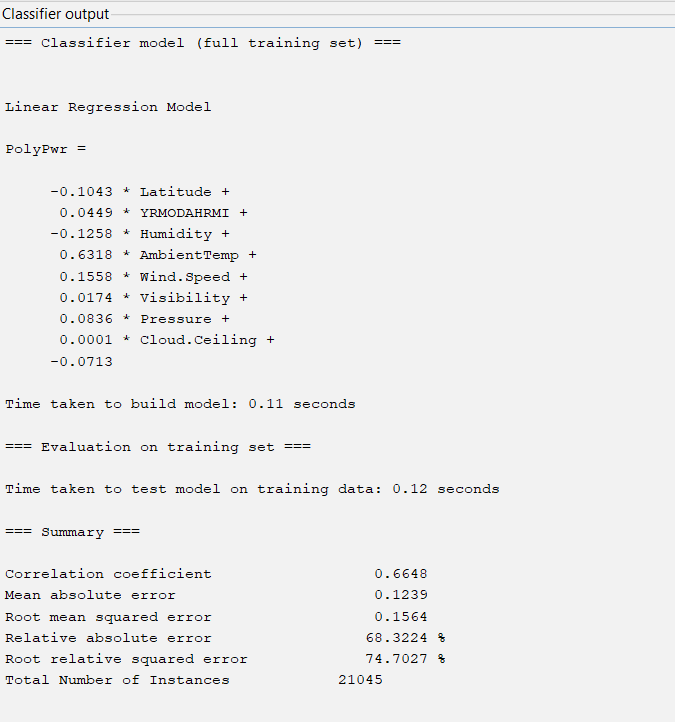
\includegraphics[width=1\linewidth]{LinReg.png}
            \caption{Linear Regression Results.}
            \label{fig:enter-label}
        \end{figure}
         
    
    \label{Figure 1}

\begin{figure}
    \centering
    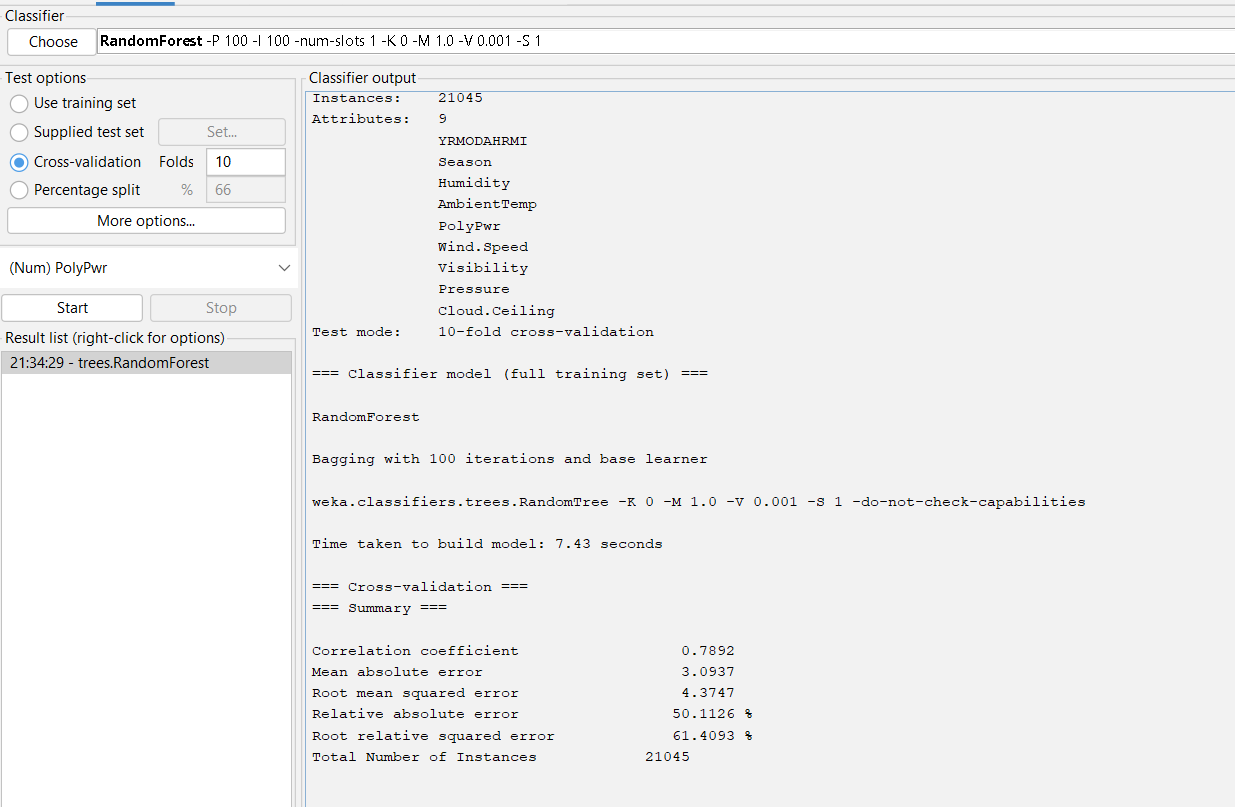
\includegraphics[width=1\linewidth]{Randomforest.png}
    \caption{ Random Forest Results.}
    \label{Figure 2}
\end{figure}

\newpage
\begin{thebibliography}{100}
\addtolength{\leftmargin}{0.2in} % sets up alignment with the following line.
\setlength{\itemindent}{-0.2in}
\bibitem{video}
“How to Build Regression Models (Weka Tutorial #1).” YouTube, YouTube, 1 Nov. 2020, www.youtube.com/watch?v=t5mylGHE2Fg.  
\bibitem{website}
Iborozan. “Iborozan/Solar: Insight Data Science Project: Predicting Photovoltaic Solar Panel Generation Using Machine Learning.” GitHub, github.com/iborozan/solar. Accessed 11 Mar. 2024. 
\bibitem{website}
Shahane, Saurabh. “Horizontal Photovoltaic Power Output Data.” Kaggle, 28 Mar. 2021, www.kaggle.com/datasets/saurabhshahane/northern-hemisphere-horizontal-photovoltaic.  
\bibitem{website}
“Rise of Solar Energy, Electric Vehicle Sales Gives Hope for Climate Goals, Report Says | CBC News.” CBCnews, CBC/Radio Canada, 26 Sept. 2023, www.cbc.ca/news/climate/iea-report-climate-emissions-1.6978343. 
\bibitem{website}
“T-Test, Chi-Square, ANOVA, Regression, Correlation...” Datatab, datatab.net/tutorial/regression. Accessed 11 Mar. 2024.  

\end{thebibliography}


\printbibliography
\printbibliography
 


\printbibliography

\end{document}
